\chapter{Trabalho realizado}
\label{chapter:work-done}

\begin{introduction}
    Neste capítulo irei abordar todo o trabalho desenvolvido durante o período de estágio, organizado em três grandes secções. Na primeira secção abordarei o trabalho realizado durante a analise de \textit{APIs} e bibliotecas, incluindo o porque da escolha final de cada uma.A segunda secção visa comentar o trabalho realizado na interface gráfica do projeto \textit{aniposture}. A terceira secção comenta o trabalho desenvolvido no respetivo \textit{backend}.
\end{introduction}

\section{Análise de bibliotecas}\label{sec:analysis}
Durante este estágio, foram-me atribuídas tarefas de análise e pesquisa, com o objetivo de identificar e selecionar as ferramentas mais adequadas que cumprissem os requisitos necessários para o desenvolvimento da aplicação. Foram, assim, realizadas duas grandes análises: a primeira sobre as \textit{APIs} de georreferenciação e a segunda nas \textit{APIs} de visualização gráfica.

\subsection{APIs georreferenciação}
Esta foi uma das primeiras tarefas que foram-me atribuídas durante o estágio. Antes de começar as comparações, foram definidos alguns requisitos fundamentais, nomeadamente a necessidade de \textit{tiles} em satelite, marcadores, bom desempenho com uma elevada quantidade de pontos e desenho de polígonos. Depois de levantados os requisitos, iniciou-se a análise comparativa entre três \textit{APIs} de georreferenciação o \textit{mapbox}, \textit{openlayers} e o \textit{google maps}.

Apesar de partilharem o mesmo objetivo, criação de mapas interativos, as três bibliotecas são consideravelmente diferentes nas suas implementações. 

\subsubsection{\textbf{OpenLayers}}\label{sec:sub_ol}

\textit{Openlayers} é o biblioteca \textit{free e Open Source} que permite a criação de mapas interativos. Disponibiliza recursos como \textit{raster tiles}, camadas vetoriais e marcadores. Por ser \textit{Open Source}, contem vários \textit{addons} criados pela comunidade que permite alargar as suas funcionalidades. Contudo, apresenta uma linha de aprendizado um pouco mais complexa do que outras alternativas e, por padrão, não contêm  nenhum \textit{tile} em satelite. 

\begin{figure}[h!]
    \centering
    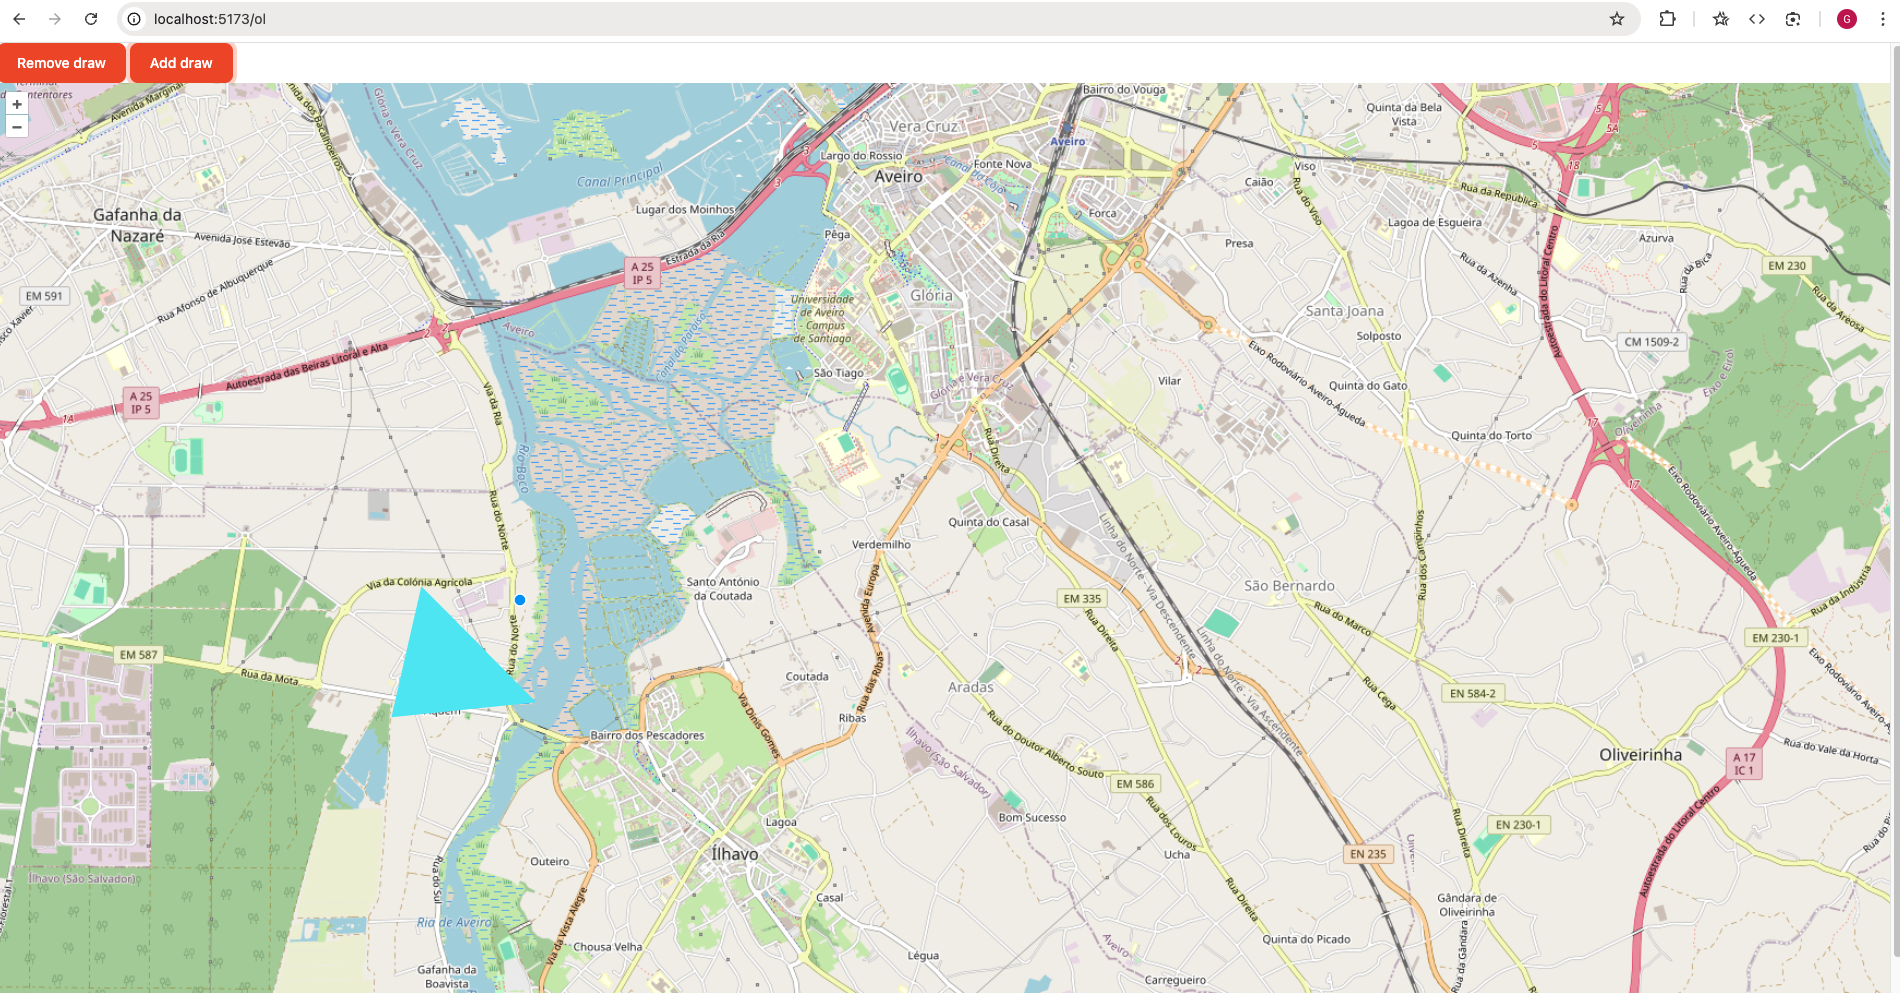
\includegraphics[width=\textwidth-1cm]{figs/ol.png}
    \caption[OpenLayers]{OpenLayers}
    \label{fig:ol}
\end{figure}

Foram ainda realizados alguns testes com opções de desenho vetorial. No entanto, o que levou o \textit{OpenLayers} não ser o escolhido foi a sua, ainda, baixa integração com \textit{WebGL}, a documentação menos completa em comparação com outras alternativas e a ausência de suporte nativo para mapa com satélite. 

\vspace{0.5cm}

\subsubsection{\textbf{Google Maps}}\label{sec:sub_gm}
O \textit{google maps} é, muito provavelmente, o sistema de mapas mais utilizado e atualizado a nível mundial. Por essa razão, foi considerada a sua utilização, tendo sido analisada a forma como é implementado e as suas funcionalidades. Inicialmente, esta solução revelou-se a mais promissora, uma vez que permite adicionar camadas vetoriais, marcadores, vista em satélite e possui um bom desempenho. 

\begin{figure}[h!]
    \centering
    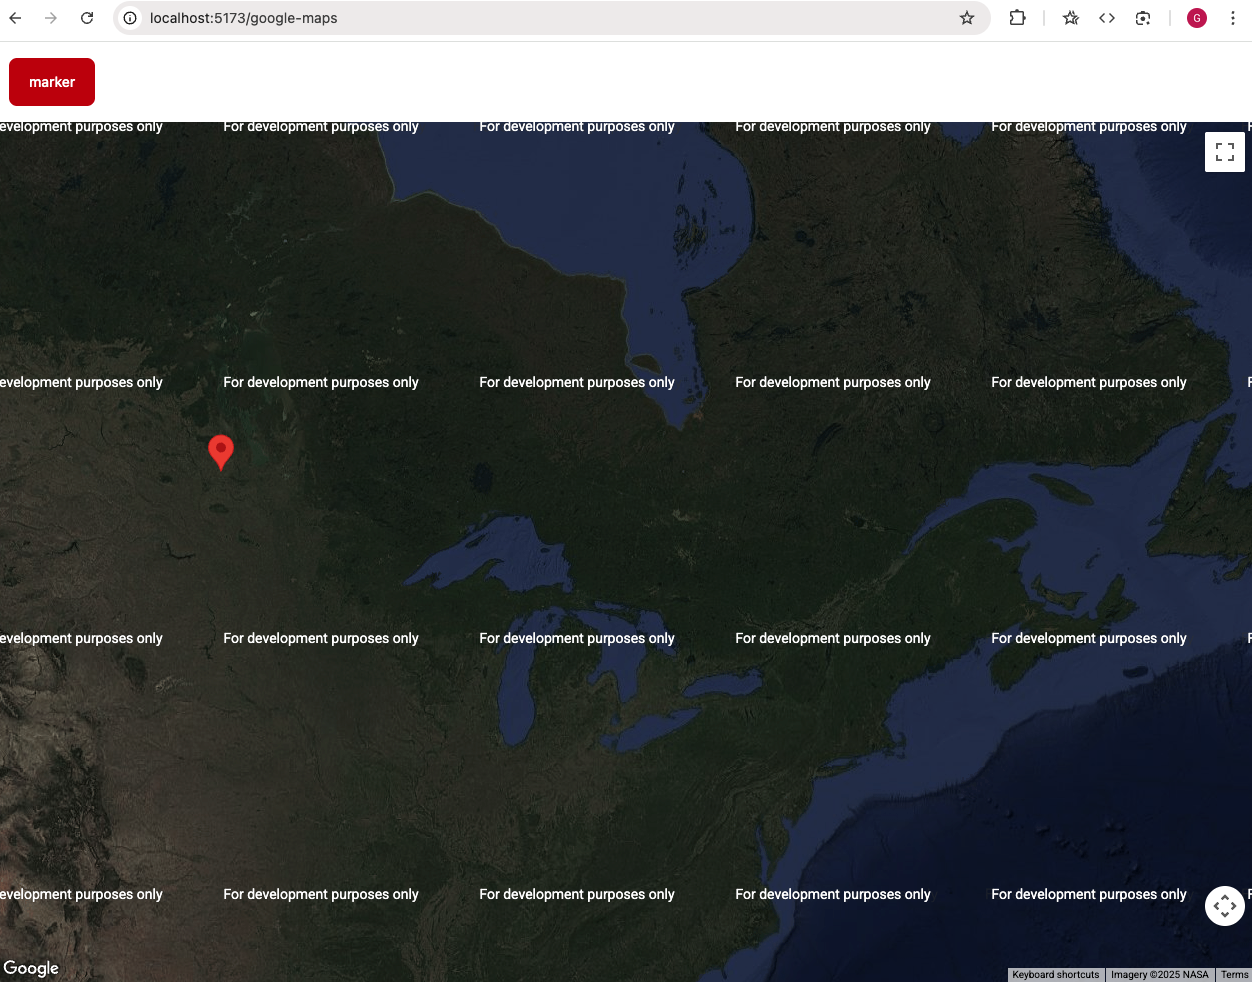
\includegraphics[width=8.95cm]{figs/gm.png}
    \caption[Google maps]{Google Maps}
    \label{fig:gm}
\end{figure}

Ao contrário do \textit{Openlayers}, \ref{sec:sub_ol}, esta é uma solução paga, que apresenta, algumas vantagens como mapas satélite mais atualizados e integração com os serviços da \textit{Google}. Contudo, o maior problema é o seu preço, consideravelmente elevado se formos comprar com outras alternativas. A \textit{Google} permite a utilização da \href{https://developers.google.com/maps/documentation/javascript}{\textit{Maps JavaScript API}} de forma gratuita até 10.000 pedidos mensais. A partir dessa quantidade começam a ser aplicadas cobranças. Devido a essa limitação o \textit{google maps} também não foi a solução escolhida.

\vspace{0.5cm}

\subsubsection{\textbf{Mapbox}}\label{sec:mapbox}
Chegamos, por fim, à opção escolhida: o \textit{Mapbox}. Esta biblioteca revelou-se a melhor entre os dois mundos, implementação inicial simples, utiliza \textit{WebGL} por padrão e disponibiliza vários tipos de \textit{tiles}, incluindo satélite. 

Embora seja uma solução paga, apresenta modelos mais em conta do que a opção da \textit{google}, a versão gratuita, contem um total de 50.000 pedidos por mês. Esta mesma quantidade de pedidos no \textit{google maps} teria um custo de cerca de 280€ mensais. Para atingir um custo parecido no \textit{mapbox}, seria necessário utilizar pelo menos 100.000 pedidos mensais. Para além do fator preço/economico, esta solução, compre todos os requisitos definidos para a nossa aplicação, juntamente de uma documentação bem estruturada.

\begin{figure}[h!]
    \centering
    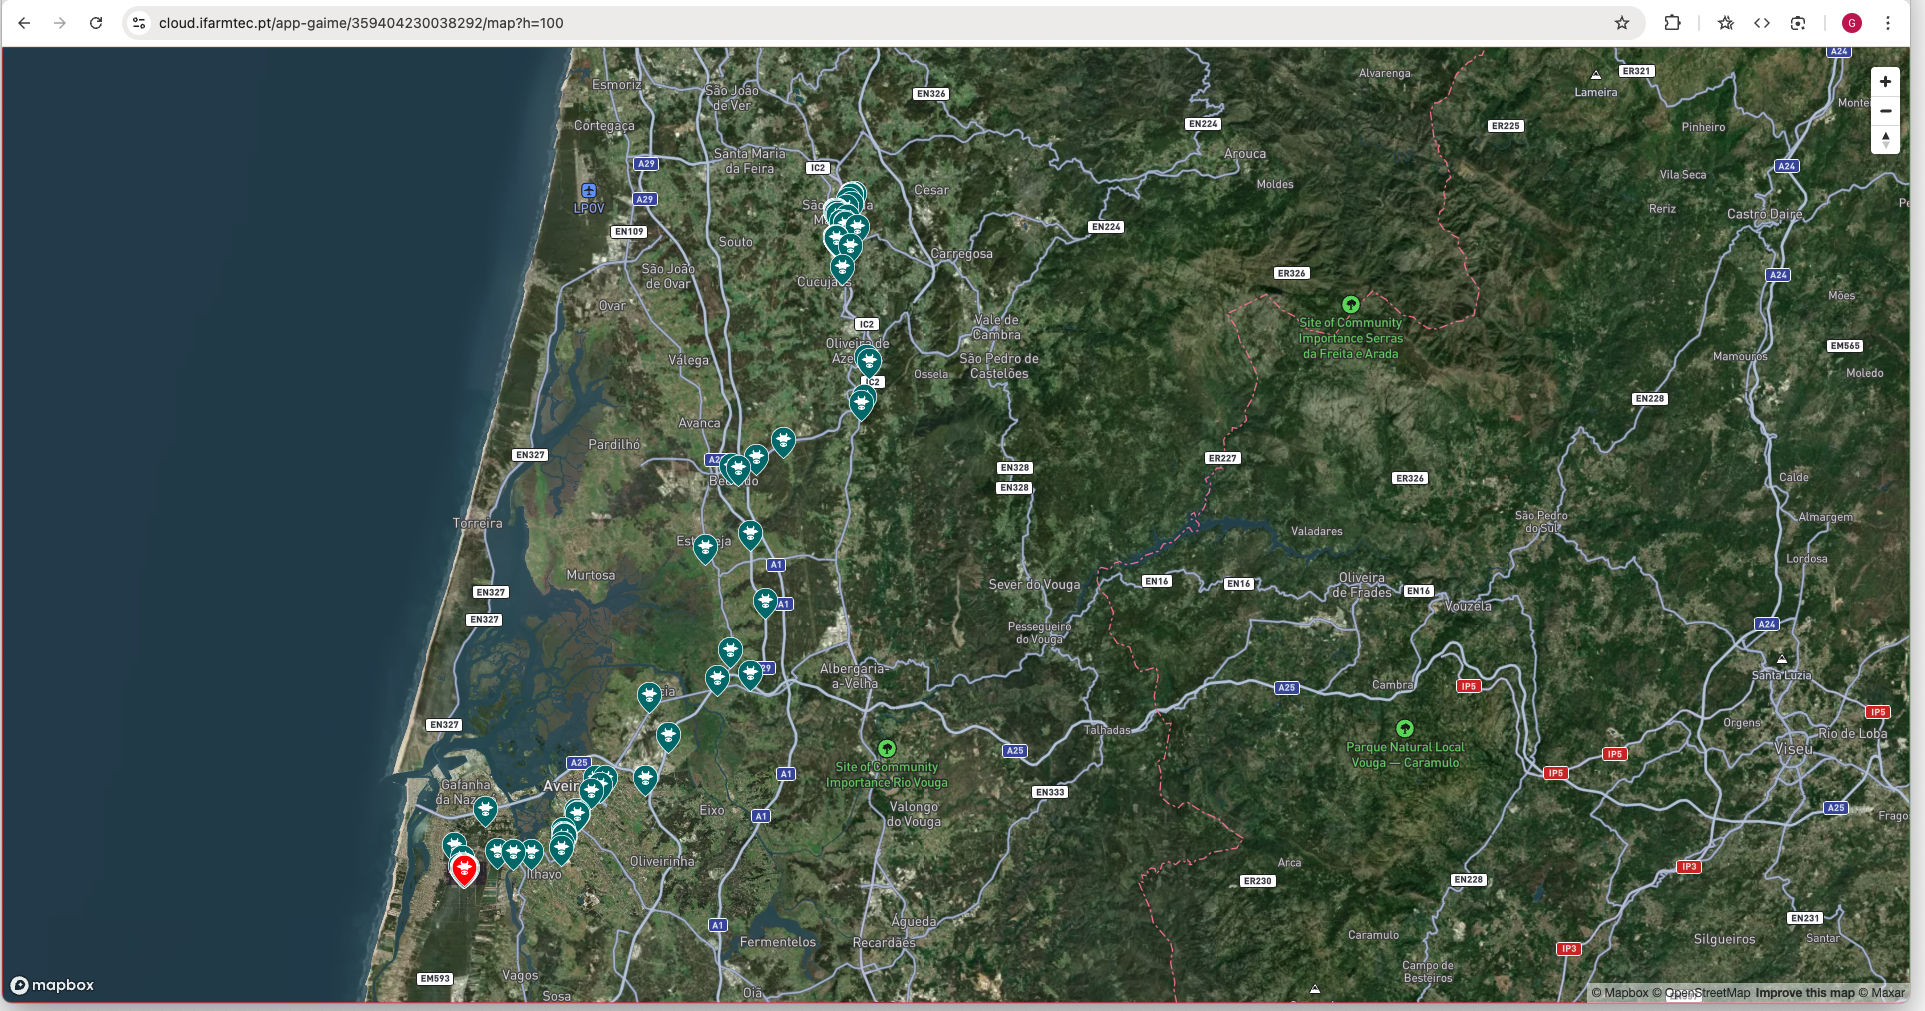
\includegraphics[width=\textwidth]{figs/mapbox.png}
    \caption[Mapbox]{Mapbox}
    \label{fig:mapbox}
\end{figure}

Tendo em conta todos os requisitos levantados, o \textit{mapbox} cumpre-os de forma exímia. Graças á sua grande comunidade, o \textit{mapbox}, dispõe vários plugins que permitem expandir significativamente as suas funcionalidades, o que acrescenta ainda mais valor à sua escolha como opção para o projeto.

% \begin{table}[h!] % [h!] is a placement specifier (here)
%   \centering % Center the table on the page
%   \caption{APIs georreferenciação, funcionalidades} % The caption for the table
%   \label{tab:api_georref} % A label to reference the table later

%   \begin{tabular}{l c c c c r} % Defines the column format: left-aligned, centered, right-aligned
%     \toprule % Top rule from booktabs
%     \textit{API} & Satelite & WebGL & Desenhar figuras & Camadas Vetoriais & Marcadores & Pago \\
%     \midrule % Mid rule from booktabs
%     \textit{Openlayers} & \ding{51} & \ding{51} & \ding{51}  & \ding{51} &  \\
%     \textit{Google maps} & 123& 123& 456 & 89.01 \\
%     \textit{Mapbox} & 123& 123& 456 & 89.01 \\
%     \bottomrule % Bottom rule from booktabs
%   \end{tabular}
% \end{table}

\clearpage

\subsection{APIs de visualização gráfica}
Após analise e avaliação das bibliotecas de georreferenciação, realizei uma pequena pesquisa e comparação na área dos gráficos.

\subsubsection{\textbf{D3js}}\label{sec:d3js}
Esta foi a biblioteca identificada pelo orientador, como uma possível opção a implementar. O \textit{d3js} não é uma biblioteca de gráficos tradicional, uma vez que possui o conceito de "gráficos". Quando visualizamos os dados com o \textit{d3js}, estamos a compor uma variedade de objetos primitivos, como linhas, círculos, retângulos, entre outros. 

Apesar de apresentar um desempenho elevado e permitir um elevado nível de interatividade, a sua utilização é consideravelmente mais complexa que outras alternativas.


\begin{figure}[h!]
    \centering
    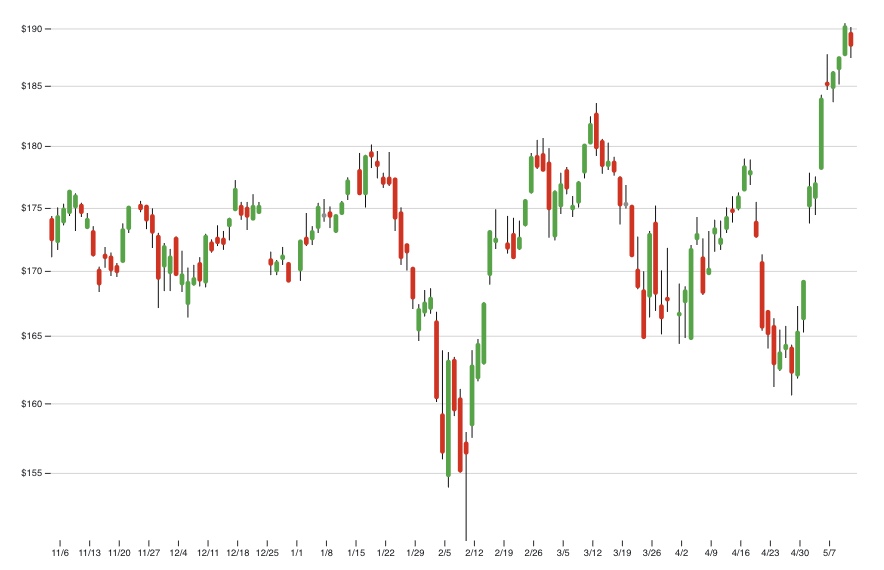
\includegraphics[width=\textwidth]{figs/d3js.png}
    \caption[Gráfico d3js]{Exemplo de gráfico criado com o d3js}
    \label{fig:d3js}
\end{figure}

\subsubsection{\textbf{ChartJs}}\label{sec:chartjs}
O \textit{chartJs} é uma das bibliotecas mais conhecidas e amplamente utilizadas no mundo \textit{JavaScript} para representação de dados.À data atual, conta com mais de \textbf{66 mil} estrelas no \href{https://github.com/chartjs/Chart.js}{\textit{github}} e é regularmente atualizada pela comunidade e pelos seus contribuidores.

Ao contrário do \textit{d3js}, \ref{sec:d3js}, o \textit{chartJs} é consideravelmente mais simples de utilizar. Trata-se de uma biblioteca que incorpora o conceito  de "gráfico", permite a visualização da informações em 8 estilos diferentes, sendo ainda responsivo. 

No entanto, essa mesma simplicidade pode ser vista como uma limitação: os gráficos, por padrão, oferecem poucos funcionalidades além da visualização básica dos informação.

\begin{figure}[h!]
    \centering
    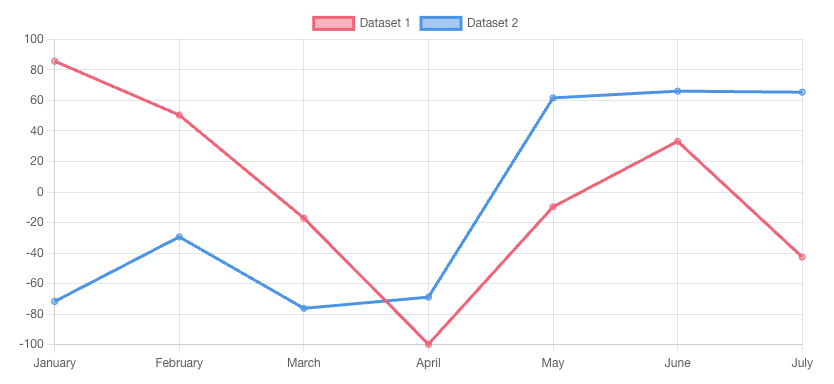
\includegraphics[width=\textwidth]{figs/chartJs.png}
    \caption[Gráfico chartJs]{Exemplo de gráfico criado com o chartJs}
    \label{fig:chartjs}
\end{figure}

\subsubsection{\textbf{Echarts}}\label{sec:echarts}
\textit{Apache Echarts} é uma biblioteca gratuita, desenvolvida no âmbito da fundação \textit{Apache}, que apresenta caracteristicas similares ao chartJs. Suporta mais de 20 tipos diferentes de gráficos, é responsivo e permite a renderização de até 10 milhões de dados em tempo real.

\begin{figure}[h!]
    \centering
    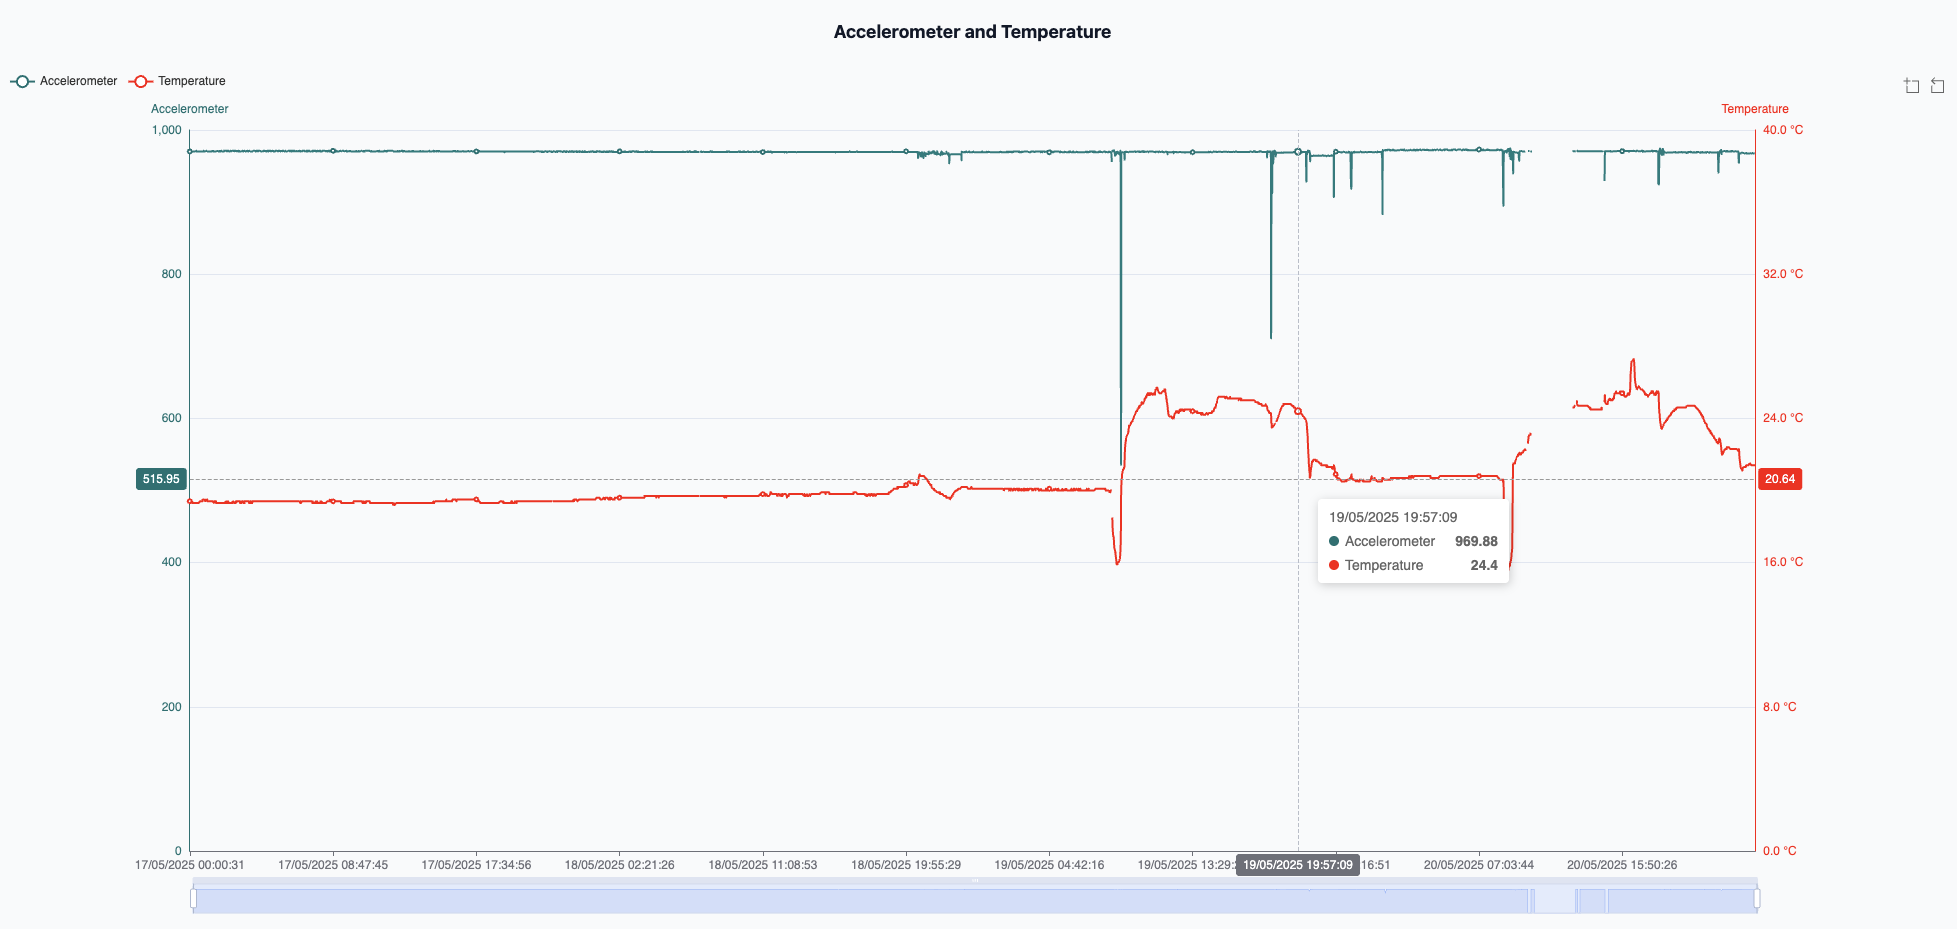
\includegraphics[width=\textwidth]{figs/echarts.png}
    \caption[Gráfico Apache Echarts]{Exemplo de gráfico criado com Echarts}
    \label{fig:echarts}
\end{figure}

O \textit{Apache Echarts} foi a solução escolhida para integrar no projeto, não apenas por apresentar um maior número de opções de visualização de dados, mas também pelas suas pelas suas funcionalidades nativas e pela elevada performance a carregar uma grandes volumes de dados. 

\clearpage
\section{Interface gráfica}\label{sec:frontend}
Nesta fase, será abordado com detalhes todo o trabalho realizado no \textit{frontend}/interface gráfica da aplicação, incluindo as dificuldades encontradas, conhecimentos adquiridos, e as tarefas realizadas durante o desenvolvimento.  

\subsection{Svelte 5}
Durante a fase de desenvolvimento, esta foi das primeiras tarefas que foram-me atribuídas. No último trimestre de 2024, a equipa responsável pelo \textit{svelte} lançou uma nova versão, que alterou conceitos fundamentais da \textit{framework}. Fui, então, encaminhado a aprender esta nova versão, testar as novas funcionalidades, compreender as principais alterações e analisar o processo de atualização um projeto desenvolvido na versão 4 para a versão 5 do svelte.